% TEMPLATE FROM:
% NAME:		swift_scijust_template.tex
% Modified on 2/17/16 by Corey Mutnik

\documentclass[letterpaper,11pt]{article}
%\documentclass[letterpaper,11pt,twocolumn]{article

\usepackage{graphics,graphicx}
%\usepackage{psfig}
\usepackage{times}
\usepackage{float}	% allows use of 'H' command



%%%%%%%%%%%%%%%%%%%%%%%%%%%%%%%%%%%%%%%%%%%%%%%%%
%%%%% Page dimensions                       %%%%%
%%%%% DO NOT CHANGE THE FOLLOWING 9 LINES!  %%%%%
%%%%%%%%%%%%%%%%%%%%%%%%%%%%%%%%%%%%%%%%%%%%%%%%%

\setlength{\textwidth}{7in} 
\setlength{\textheight}{9.5in}
\setlength{\topmargin}{-0.2in} 
\setlength{\oddsidemargin}{-0.2in}
\setlength{\evensidemargin}{-0.2in} 
\setlength{\headheight}{0in}
\setlength{\headsep}{0in} 
\setlength{\hoffset}{0in}
\setlength{\voffset}{0in}


%%%%%%%%%%%%%%%%%%%%%%%%%%%%%%%%%%
%%%%% Section heading format %%%%%
%%%%%%%%%%%%%%%%%%%%%%%%%%%%%%%%%%

\makeatletter
\renewcommand{\section}{\@startsection%
{section}{1}{0mm}{-\baselineskip}%
{0.5\baselineskip}{\normalfont\Large\bfseries}}%
\makeatother



% DEFINE BOX ENVIRONMENT %%%%%%%%%%%%%%%%%%%%%%%%%%%%%%%%%%%%%%%%%%%%%%%%%%%%%%%%%%%%%%%%%%%%%%%%%%%%%%
%%%%%%%%%%%%%%%%%%%%%%%%%%%%%%%%%%%%%%%%%%%%%%%%%%%%%%%%%%%%%%%%%%%%%%%%%%%%%%%%%%%%%%%%%%%%%%%%%%%%%%%
\newsavebox\FrameBox
\newenvironment{Frame}{%
  \noindent\setbox\FrameBox\hbox\bgroup\minipage{1.01\textwidth}\parskip\baselineskip\ignorespaces
}{%
  \endminipage\egroup\fbox{\box\FrameBox}\par
}
%%%%%%%%%%%%%%%%%%%%%%%%%%%%%%%%%%%%%%%%%%%%%%%%%%%%%%%%%%%%%%%%%%%%%%%%%%%%%%%%%%%%%%%%%%%%%%%%%%%%%%%
%%%%%%%%%%%%%%%%%%%%%%%%%%%%%%%%%%%%%%%%%%%%%%%%%%%%%%%%%%%%%%%%%%%%%%%%%%%%%%%%%%%%%%%%%%%%%%%%%%%%%%%



\begin{document}
\pagestyle{plain}
\pagenumbering{arabic}

\begin{center} 
\bfseries\uppercase{\Large{University of Hawaii $\bullet$ Institute for Astronomy} \\ 
\large{Research Proposal -- Observing Time Request}}
\end{center}
\vspace{-0.3cm}


\iffalse
	% box around names, emails, and institution
	\noindent\fbox{\linespread{1.5}
		\parbox{\textwidth}{\bf{
				Names: {Daichi Hiramatsu} \& {Corey Mutnik} \\
				E-mails: dhiramat@hawaii.edu \& cmutnik@hawaii.edu\\
				Institution/Dept: UH
			}
		}
	} 
	~\\ %this is here to make gap between boxes
	% box around program titles
	\noindent\fbox{\linespread{1.5}
		\parbox{\textwidth}{\bf{
				Program Title\\
				A. Measuring the Milky Way\\
				B.\\
				C.
			}
		}
	} 
\fi


\noindent\fbox{\linespread{2}
  \parbox{\textwidth}{\bf{
	\begin{minipage}{0.5\textwidth}
		\begin{flushleft}
	    	\subsection*{Author$^{*}$~:~Daichi~Hiramatsu}
	    	%\subsection*{Author$_{1}$~:~Daichi~Hiramatsu\\E-mail$_{1}$~:~dhiramat@hawaii.edu}
		\end{flushleft}
	\end{minipage}
  \hfill
	\begin{minipage}{0.5\textwidth}
		\begin{flushright}
	    	\textbf{\large Author$^{\dagger}$~:~Corey Mutnik~~}\\[1.5cm]
		\end{flushright}
	\end{minipage}
	\begin{minipage}{0.5\textwidth}
		\begin{flushleft}
			\subsection*{E-mail$^{*}$~:~dhiramat@hawaii.edu}
		\end{flushleft}
	\end{minipage}
  \hfill
	\begin{minipage}{0.5\textwidth}
		\begin{flushright}
	    	\textbf{\large E-mail$^{\dagger}$~:~cmutnik@hawaii.edu~~}\\[1.5cm]
		\end{flushright}
	\end{minipage}

	\subsection*{Institution/Dept$^{*,\dagger}$~:~UH}
  }
 }
}

~\\ % for gap between frames

\begin{Frame}
\noindent {\bf \\Abstract}
\smallskip\\


% can report variable stars to AAVSO:
% https://www.aavso.org/how-report-new-variable-star-discoveries

\end{Frame}
~\\
\section*{TELESCOPE TIME REQUESTED}

\section*{COLLABORATORS}
\begin{table}[H]\label{tab:collabs}
	\begin{center}
		%\caption{\it \small{[title]}}
		\resizebox{\columnwidth}{!}{%
	\begin{tabular}{ | c | c | c | c | } \hline
		Name & Institution & E-mail & Program(s) \\ \hline
		 Jeff & UH & & \\ \hline
		 Marielle & UH & & \\ \hline
		 Connor & IfA & & \\ \hline
		 JT & IfA & & \\ \hline
		 & & & \\ \hline
		 & & & \\ \hline
		 & & & \\ \hline
		 & & & \\ \hline
		 & & & \\ \hline
	\end{tabular}
	}
	\end{center}
\end{table}



\section{SCIENTIFIC JUSTIFICATION}

\subsection{Immediate Objective}
Using various data reduction techniques, we will measure the size, shape, and age of the spiral arms located on the Milky Way galaxy. To determine the size and shape of particular spiral arms, variable star distributions must be spatially mapped.  
%Distributions of variable stars allows for the determination of both size and shape of 
The number distribution of variable stars will give insight into the age of our galaxy.

\begin{itemize}
	%\item{} Use gri data to identify variable Stars 		
	%\item{} Use Period-Luminosity relationship to get distance 
	%\item{} Map 3D spatial distribution
	\item{} Distance Equation with reference
	\item{} Determine deviation of variable stars from model
	\item{} Variations arise from non-gravitational effects
	\item{} Figure out dark matter distribution
	\item{} include - Plot of known var star distributions in spiral arms
	\item{} possibly make figures below, side by side
\end{itemize}
Subtraction of gri data will cause transient objects to emerge.  
%Variable stars have distinct light curves. Analysis of subtracted gri data will lead to classification of variable stars.
Distinct light curves will lead to the identification of variable stars.  
%The number of variable stars relative to the total number of stars is less than 1\% [CITE WIKI], making 
Variable stars comprise under 1\% of the total number of observable stars Allen et al. (2016), making it possible to analyze all of the data collected by the gri project.


A H-R Diagram of pulsating variable stars is shown by Figure~\ref{fig:var-star-hr} Turner et al. (2012).


\subsection{Scientific Rationale}
%~\\ Data Processing
%\begin{itemize}
	%\item{} how we pick variable stars (RR Lyrae, Type 1 Cephedis, and Type 2 Cephedis) from gri data
	%\item{} distinguished by unique light curves
	%\item{} \# var stars is less than 1\% of total stars - this is how we will deal with vast amount of data
	%\item{} ref - `stellar classifications' on wikipedia
%\end{itemize}
Of the different types of variable stars, we will focus on RR Lyrae, Type 1 Cephedis, and Type 2 Cephedis.  These pulsating variables have well established absolute magnitudes B. et al. (2012).  From this the luminosity is known, permitting the distance to each star to be calculated using Period-Luminosity (PL) relationship.

RR Lyrae have short periods, $1.5 - 24$ hours, and are generally classified as stars with spectral type A.  On average, absolute magnitudes of RR Lyrae stars fall between 0.6-0.7 Tsujimoto et al. (1998). Using the distance modulus assuming no ISM extinction yields the upper limit on RR Lyrae distance measurements of $7.9$ kpc with $m=15$ (photometric accuracy of $4\%$). Figure~\ref{fig:plrelationrrlyrae} shows the PL relationship for variable stars classified as RR Lyrae Ngeow et al. (1998) (\textit{how do we calibrate different band passes?}).

~[DISCUSS Type 1 Cephedis, and Type 2 Cephedis]
~[DISCUSS DIFFERENCE IN ALL 3 VAR TYPE'S LIGHT CURVES - POSSIBLY SHOW EXAMPLES]

\begin{figure}[htb!]
  \begin{center}
\centerline{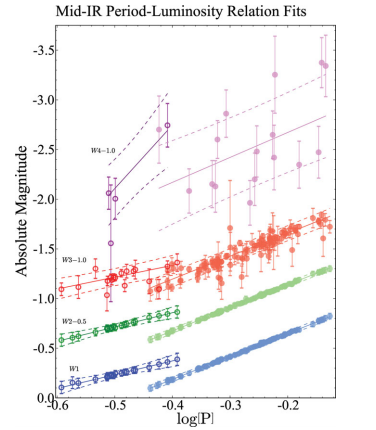
\includegraphics[width=3in]{figures/PL_relation}}
\caption{\it \small{Period-Luminosity relationship of RR Lyrae variable stars. \label{fig:plrelationrrlyrae}}}
  \end{center}
\end{figure}
\begin{figure}[htb!]
  \begin{center}
\centerline{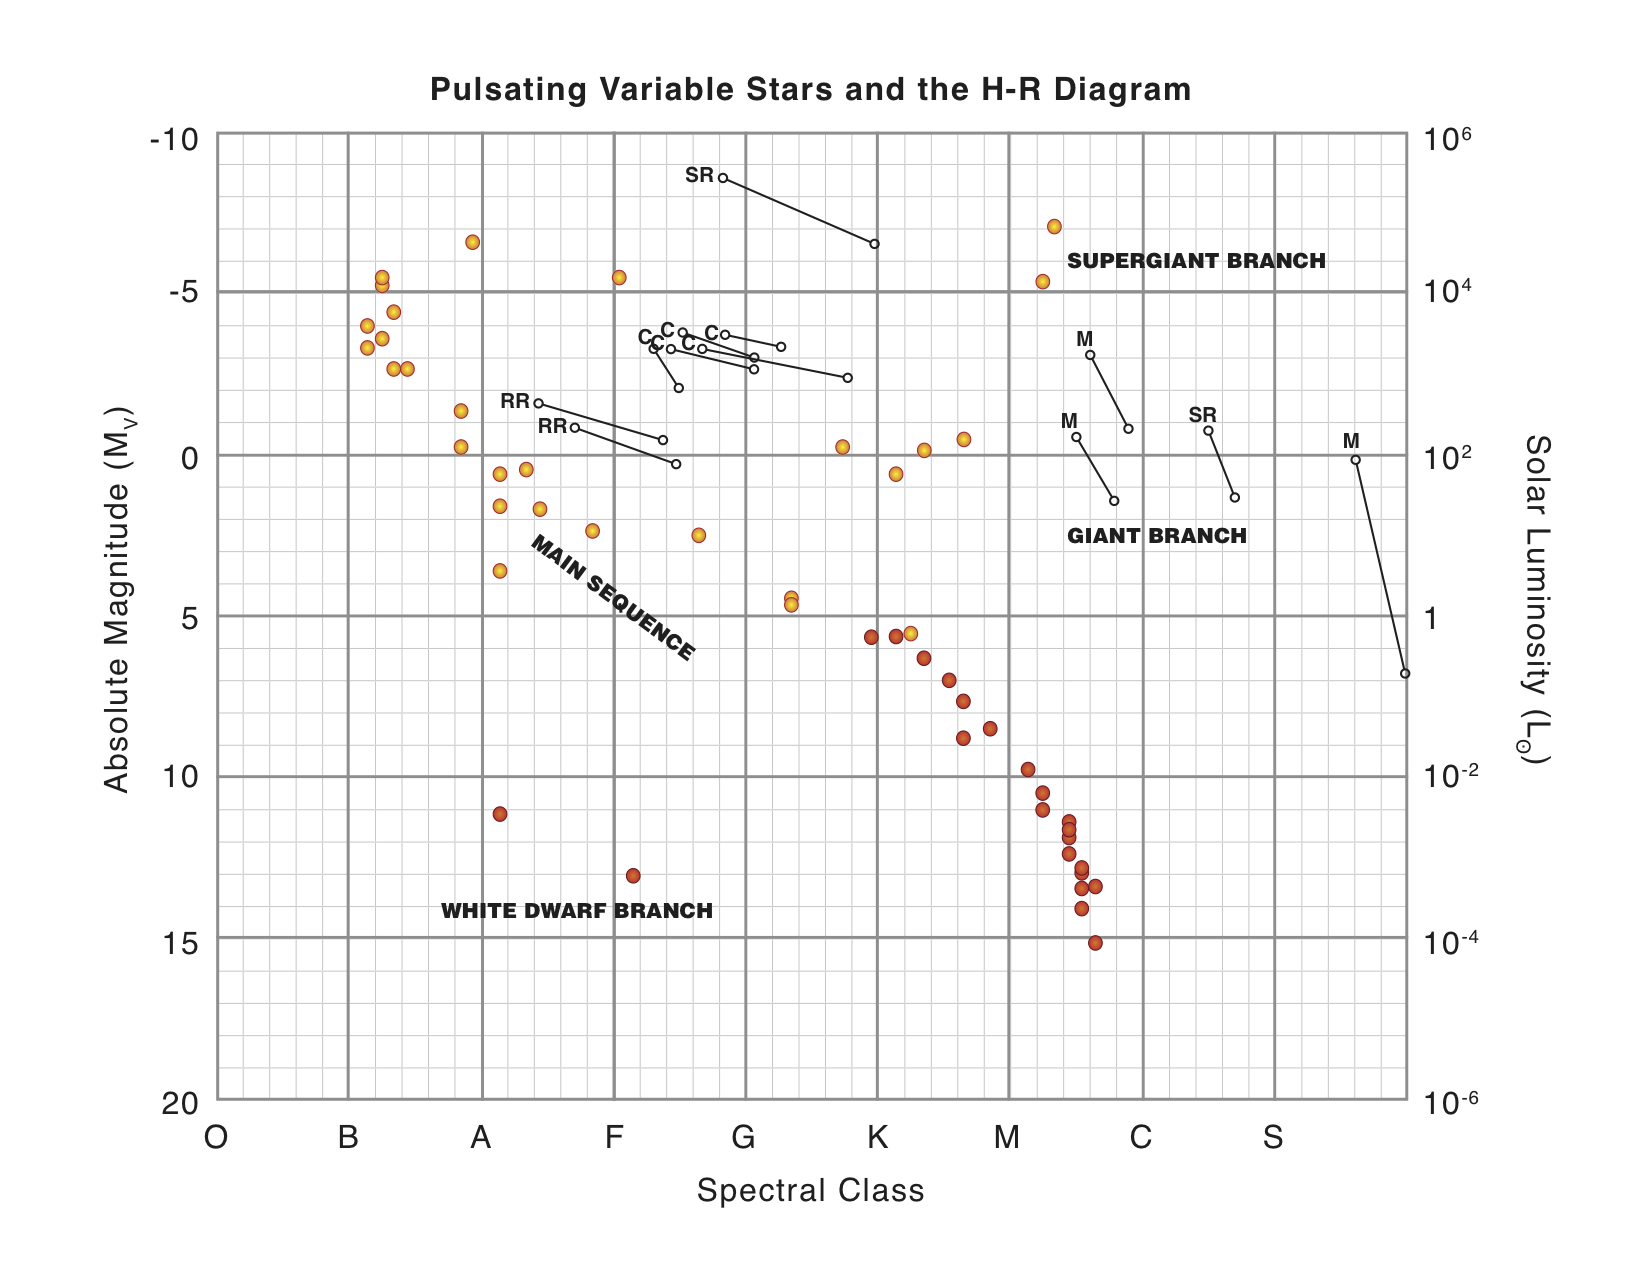
\includegraphics[width=3in]{figures/var_star_HR.png}}
\caption{\it \small{HR-Diagram: Pulsating Variable Stars. \label{fig:var-star-hr}}}
  \end{center}
\end{figure}


Near the galactic center, ISM is dense, and the number density of stars is high, which makes optical investigations quite difficult. Figure ~ \ref{fig:gas} shows the distribution of gasses in the Milky Way (Nakanishi and Sofue 2015). In order to determine the spiral arm structure of the Milky Way galaxy, we avoid the galactic center. To take into account for the ISM extinction, we use the ratio of total to selective extinction $R = \frac{1}{(\tau_{1} / \tau_{2}) -1} = \frac{1}{(\lambda_{eff,1} / \lambda_{eff,2})^{-1} \, -1}$ assuming the optical depth $\tau \propto \lambda^{-1}$ according to the Mie scattering. 

\begin{figure}[htb!]
  \begin{center}
\centerline{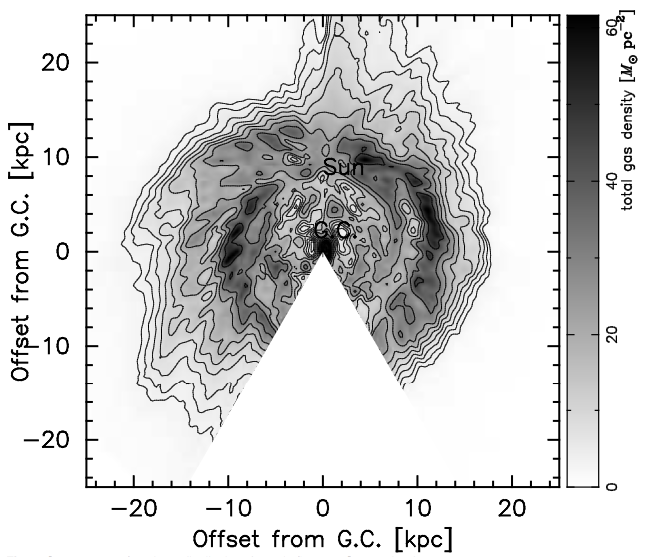
\includegraphics[width=3in]{figures/Gas.png}}
\caption{\it \small{Column density distribution of the sum of HI and H$_2$ gases. \label{fig:gas}}}
  \end{center}
\end{figure}



\section*{References}

\noindent\smallskip{\small
Allen, S.\ et al., 2016. (n.d.). The Classification of Stellar Spectra. Retrieved February 15, 2016, from $http://www.star.ucl.ac.uk/~pac/spectral_classification.html$ \\}

\noindent\smallskip{\small
B.\ et al., 2012. Types of Variables | AAVSO. Retrieved February 16, 2016, from https://www.aavso.org/types-variables \\}

\noindent\smallskip{\small
Ngeow, C.\ et al., 2013. "Distance Determination From The Cepheid And RR Lyrae Period-Luminosity Relations". \textit{Proc. IAU} 9.S301: 123-128. Web. 18 Feb. 2016. \\}

\noindent\smallskip{\small
Tsujimoto\ et al., 1998. The Absolute Magnitude of RR Lyrae Stars Derived from the [ITAL]Hipparcos[/ITAL] Catalogue. \textit{The Astrophysical Journal, 492}(1). Retrieved February 15, 2016. \\}

\noindent\smallskip{\small
Turner, R.\ et al., 2012. H-R Diagram Education Materials | AAVSO. Retrieved February 14, 2016, from https://www.aavso.org/hr-diagram-education-materials \\}

\noindent\smallskip{\small
Nakanishi, H. and Sofue, Y., 2015. Three-Dimensional Distribution of the ISM in the Milky Way Galaxy: III. The Total Neutral Gas Disk. \textit{Publ. Astron. Soc. Japan (2014) 00(0), 1–14}. Retrieved February 15, 2016. \\}

\section*{TECHNICAL JUSTIFICATION}


We request $10.3$ hours using Pathfinder to obtain g, r, and i imaging for variable stars in the galactic plane.

\vspace{3mm} %3mm vertical space

\noindent The typical pulsation period of RR Lyrae is in a range of $1.5$ hours to $24$ hours. To reconstruct a $1.5$ hours period, we need to image a RR Lyrae at least twice in one period according to the sampling theorem (\textit{sampling rate vs error?}). With the exposure time of $30$ seconds and readout time of $8$ seconds, the sky coverage rate is $948$ deg$^2$/hour. To cover the galactic plane and avoid the galactic center, we choose a region with galactic latitude of $\pm 2 ^\circ$ and galactic longitude of $70 ^\circ$ to $290 ^\circ$ (\textit{from the gri project, we should be able to choose smaller patches with variable stars on the galactic plane; more points in one period}). The coverage rate and angular size of the field yield the one observation time of $1.14$ hours. We want $3$ band passes with $3$ pulsation periods each to take into account the ISM extinction (\textit{number of periods vs error?}), so we request the total observational time of $10.3$ hours.

\vspace{3mm} %3mm vertical space

\noindent The SNRs of g, r, and i bands with $m_g = m_r = m_i = 15$ are $26.11$, $26.31$, and $20.67$, respectively. We use relative intensity to measure pulsation periods, so this photometric accuracy of $4 \%$ should be enough (\textit{photometric accuracy vs error?}).






\end{document}